\documentclass[10pt,a4paper]{article}
\usepackage[utf8]{inputenc}
\usepackage{amsmath,amssymb,amsfonts}
\usepackage{geometry}
\geometry{a4paper, margin=0.6in}
\usepackage{booktabs}
\usepackage{graphicx}
\usepackage{microtype}
\usepackage{charter}
\usepackage[colorlinks=true, linkcolor=blue, citecolor=blue, urlcolor=blue]{hyperref}
\usepackage{multicol}

\pagestyle{empty}

\begin{document}

\begin{center}
    {\LARGE \textbf{Nonlinear Liquidity Reversion (NVR) Strategy}} \\
    \vspace{0.05in}
    {\large \textbf{Proprietary Quantitative Research -- Strategy Fact Sheet}} \\
    \vspace{0.05in}
    Confidential -- Internal Distribution Only -- July 2026
\end{center}

\vspace{0.1in}
\hrule
\vspace{0.1in}

\begin{multicols}{2}

\section*{Strategy Profile}
\textbf{Investment Objective:} Exploit overnight mean-reversion anomalies within the Russell 3000 universe, using volume-weighted execution algos to extract liquidity premium while minimizing price slippage.\\
\textbf{Portfolio Focus:} US Small/Micro-Cap Equities.\\
\textbf{Position Sizing:} Inverse Volatility (Risk-Parity).\\
\textbf{Holding Period:} 3-Day Tranche Rebalancing.\\
\textbf{Leverage:} 1.0x (No Margin Loans/Interest).\\
\textbf{Execution:} 3-Hour VWAP Algo (Exits).

\columnbreak

\section*{Key Performance Metrics (2020--2026)}
\begin{tabular}{lr}
\toprule
\textbf{Metric} & \textbf{Value} \\
\midrule
Net Sharpe Ratio & \textbf{1.492} \\
Net Annualized Return (CAGR) & \textbf{91.04\%} \\
Max Drawdown & -57.45\% \\
Inception Date & January 2020 \\
Terminal Capacity Limit & \$2.5M -- \$3.0M \\
Min starting Capital & \$10,000 \\
\bottomrule
\end{tabular}

\end{multicols}

\vspace{0.05in}
\hrule
\vspace{0.1in}

\section*{Year-by-Year Performance Metrics (2020--2026)}
\begin{center}
\begin{tabular}{ccccc}
\toprule
\textbf{Year} & \textbf{Net Sharpe} & \textbf{Net Return} & \textbf{Max Drawdown} & \textbf{Trading Days} \\
\midrule
2020 & 1.578 & 135.55\% & -40.36\% & 253 \\
2021 & 1.188 & 56.25\% & -23.95\% & 252 \\
2022 & 0.022 & -15.49\% & -42.21\% & 251 \\
2023 & 2.329 & 179.54\% & -52.34\% & 250 \\
2024 & 4.078 & 1,325.61\% & -20.10\% & 252 \\
2025 & 1.660 & 149.87\% & -34.79\% & 250 \\
2026 (YTD) & 0.672 & 22.25\% & -23.48\% & 106 \\
\bottomrule
\end{tabular}
\end{center}

\vspace{0.05in}
\hrule
\vspace{0.1in}

\section*{Strategy Equity Curve (PnL Growth)}
\begin{center}
    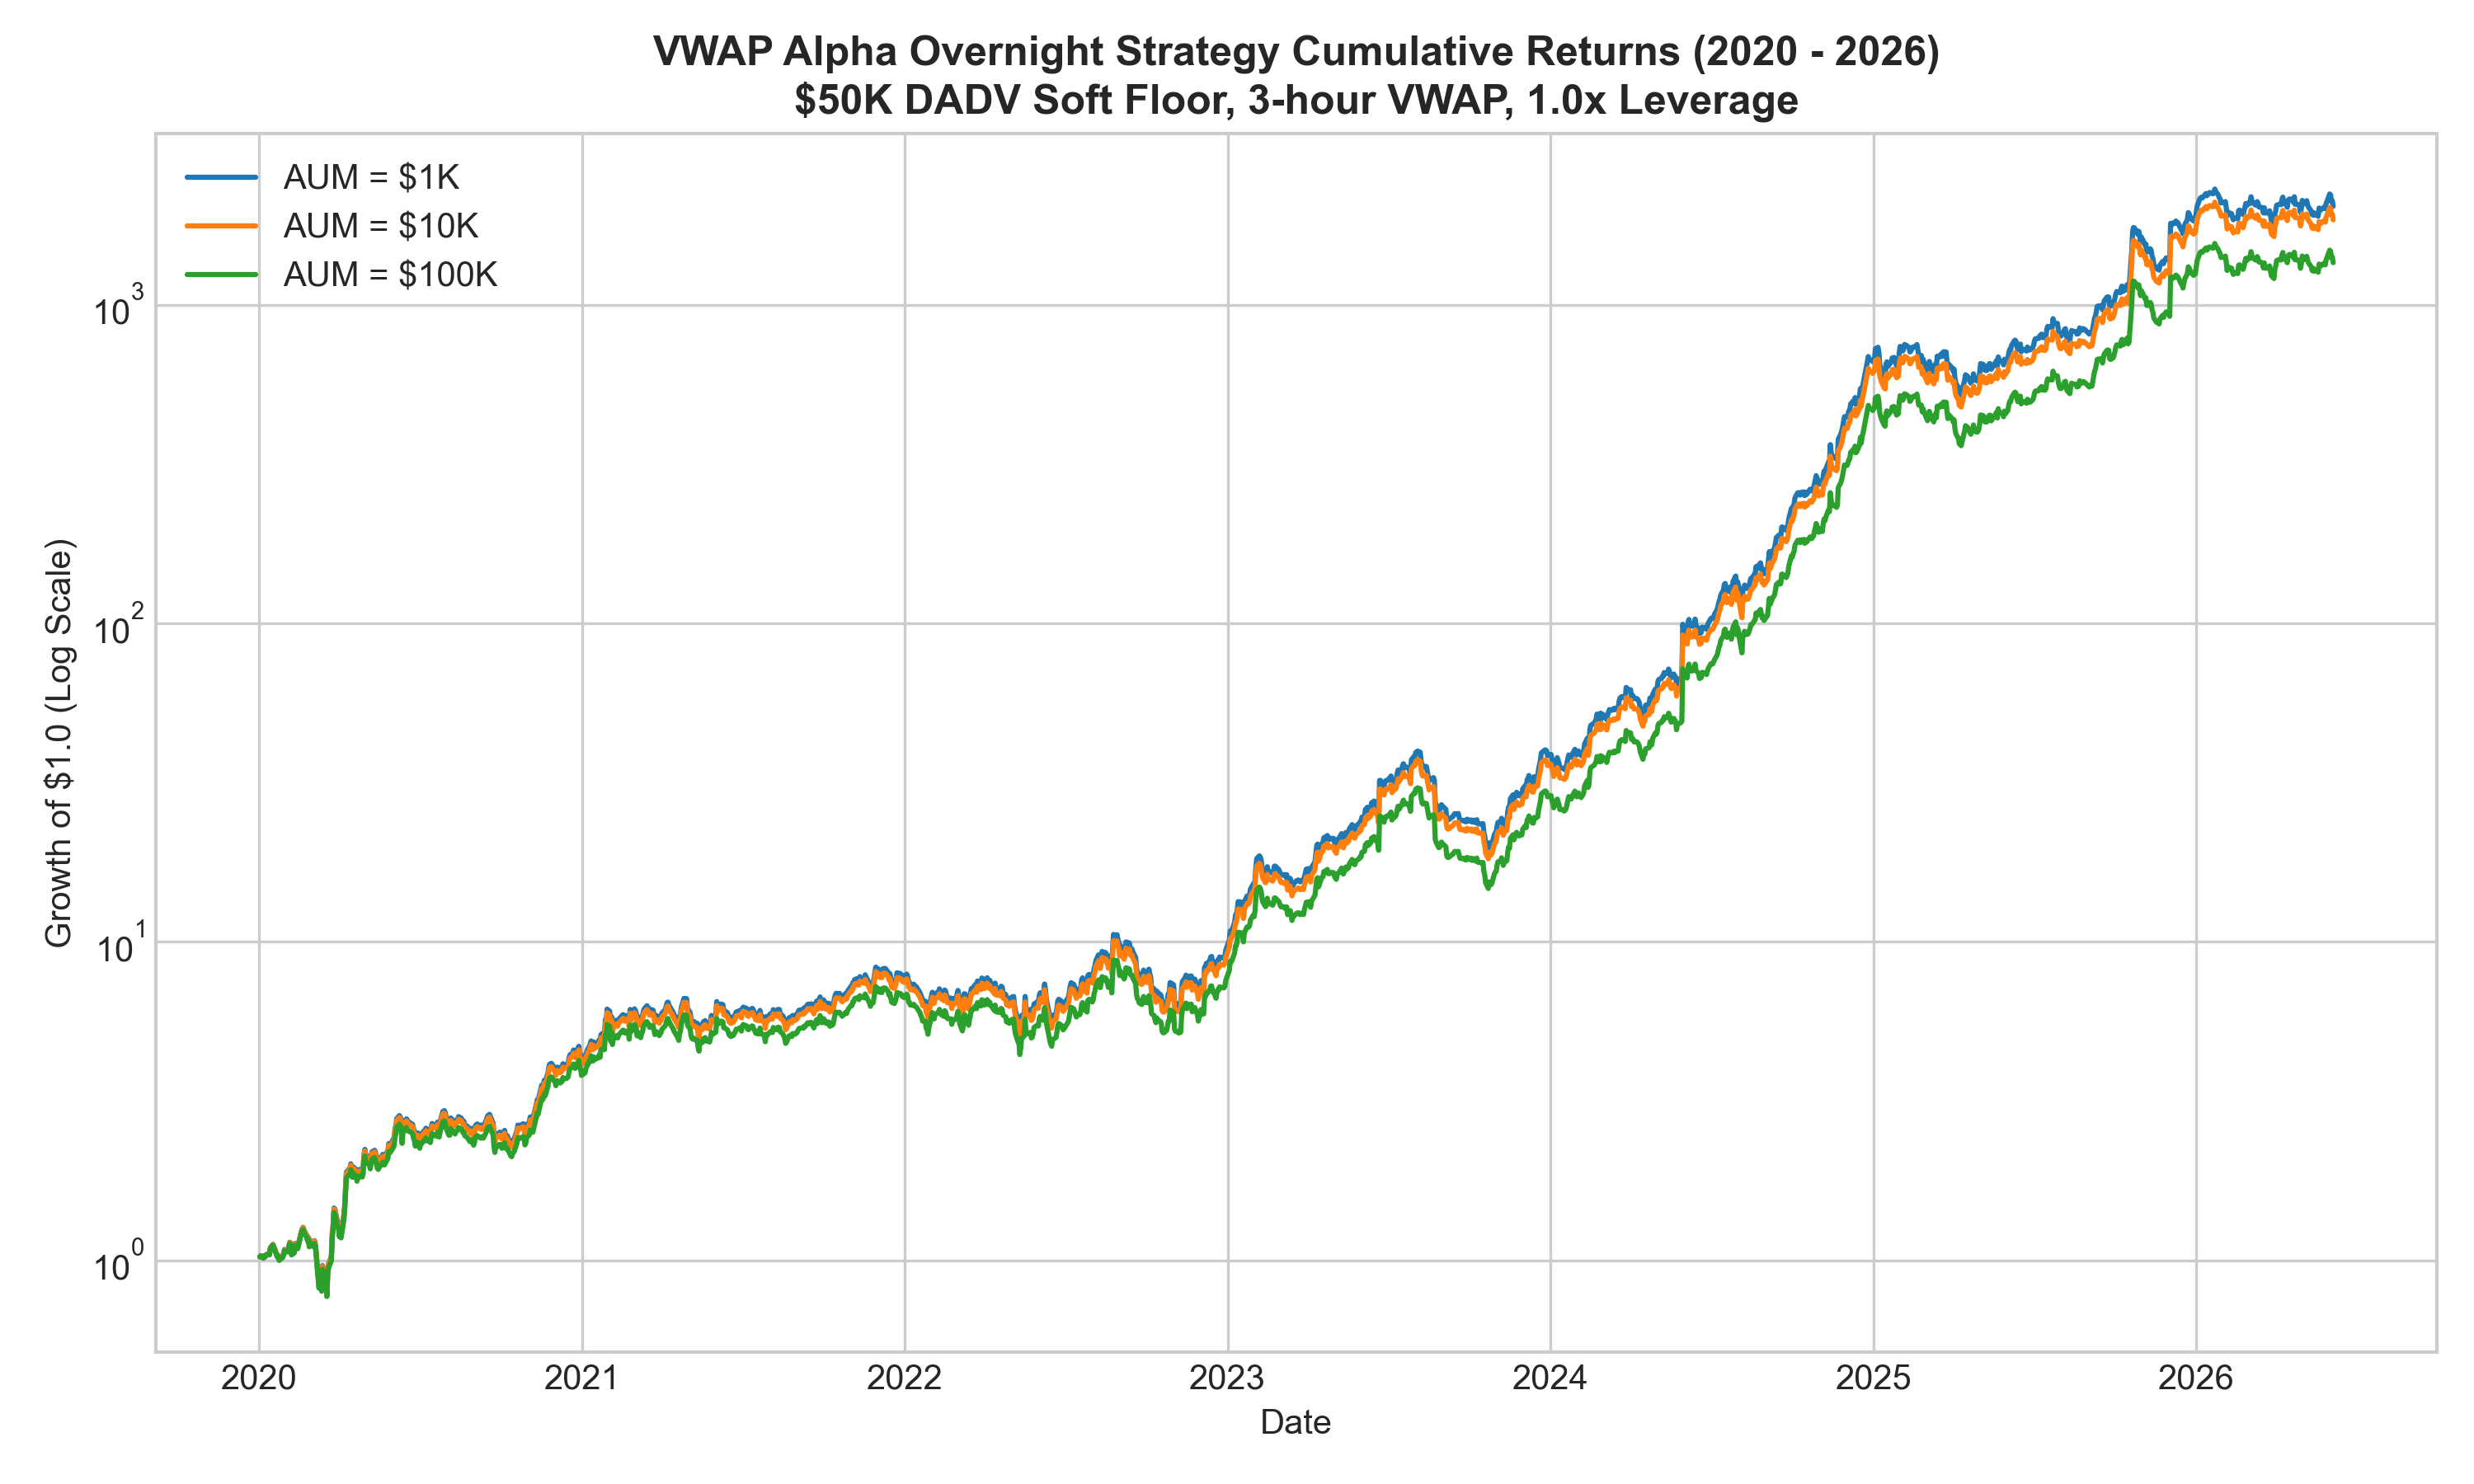
\includegraphics[width=0.85\textwidth]{pnl_chart_2020_2026.png} \\
    \small{\textit{Figure 1: Growth of \$1.0 invested since Jan 2020 (Log Scale). Net of 3-hour VWAP slippage, commissions, and spreads.}}
\end{center}

\vspace{0.05in}
\hrule
\vspace{0.1in}

\section*{Key Risk Controls \& Operational Guards}
\begin{itemize}
    \item \textbf{Soft Liquidity Floor:} Dynamic thresholding (\$50K ADDV soft floor under \$100K AUM, shifting to \$1.0M ADV above \$100K AUM) to ensure execution fills and avoid nano-cap liquidity traps.
    \item \textbf{Beta/Regime Filter:} Strategy halts trading and rotates to Cash when the S&P 500 trades below its 200-day simple moving average to protect capital during trending bear markets.
    \item \textbf{Nonlinear Market Impact Management:} Exits are routed using a 3-hour VWAP algorithm to keep the trading footprint within the cheapest part of the square-root market impact curve.
\end{itemize}

\end{document}
